\documentclass[dvipdfm,serif,mathserif]{beamer}
\usepackage{color}
\usepackage{amsmath, amsfonts, epsfig, xspace}
\usepackage{algorithm,algorithmic}
\usepackage{pstricks,pst-node}
\usepackage{multimedia}
\usepackage[normal,tight,center]{subfigure}
\usepackage[boldfont,slantfont,CJKnumber]{xeCJK}

\setCJKmainfont[BoldFont=Adobe Heiti Std]{Adobe Song Std} % 设置默认的中文字体
\setCJKfamilyfont{kai}{Adobe Kaiti Std}

\definecolor{darkgreen}{rgb}{0,.39,0}

\renewcommand{\today}{\number\year 年 \number\month 月 \number\day 日}
\usetheme{Montpellier}

\definecolor{steelblue}{rgb}{.275,.51,.71}
\definecolor{lpink}{rgb}{.991,.711,.754}
\definecolor{mygray}{gray}{0.92}
\definecolor{darkblue}{rgb}{0,0,.5}
\definecolor{darkgreen}{rgb}{0,.39,0}
\definecolor{hgray}{gray}{.5}
\definecolor{lgray}{gray}{.8}

\graphicspath{{data/}} %%图片路径
%  \DeclareGraphicsExtensions{.}
\hypersetup{pdfpagemode={FullScreen}} % 全屏幕

\begin{document}

% \author{颜开}
\title{The 第二次 Talk of \textcolor{darkgreen}{iMath}}
\date{\today}
\author{Jerry Mouse}

\begin{frame}
  \titlepage
\end{frame}
\begin{frame}\frametitle{目录}
\tableofcontents
\end{frame}


\AtBeginSection[] {
  \frame<handout:0> {
    \frametitle{目录}
    \tableofcontents[current]
  }
}

\section{来点实际的}


\begin{frame}
\frametitle{iMath主页}
 \href{http://i-math.appspot.com/}{http://i-math.appspot.com/}
\end{frame}

\begin{frame}
  \frametitle{效果图}
  \includegraphics[width=\textwidth]{screenshot.ps}
\end{frame}


\section{俺们干了什么?}

\begin{frame}
  \frametitle{经典回放}
\begin{itemize}
 \item[时间] Now -  5月10日
 \item[框架] 马马虎虎作出框架,注重定义接口
 \item[工具] 基本工具要有,但不多
\end{itemize}
\end{frame}

\subsection{团队方面}

\begin{frame}
  \frametitle{三人组}
形成一个会付出大量精力三人组来对这个项目负责。
\begin{itemize}
 \item 功能设计师:陶
\item 架构师:颜
\item 外观设计师(竞选中...)
\end{itemize}
\end{frame}

\begin{frame}
  \frametitle{合作方面}
\begin{center}
 \item 胶冻团队是第一目的
\end{center}
\end{frame}

\subsection{功能方面}

\begin{frame}
  \frametitle{Tabs}
\begin{itemize}
 \item 概率运算
\item 分布运算
\end{itemize}
\end{frame}


\begin{frame}
  \frametitle{概率小工具}
  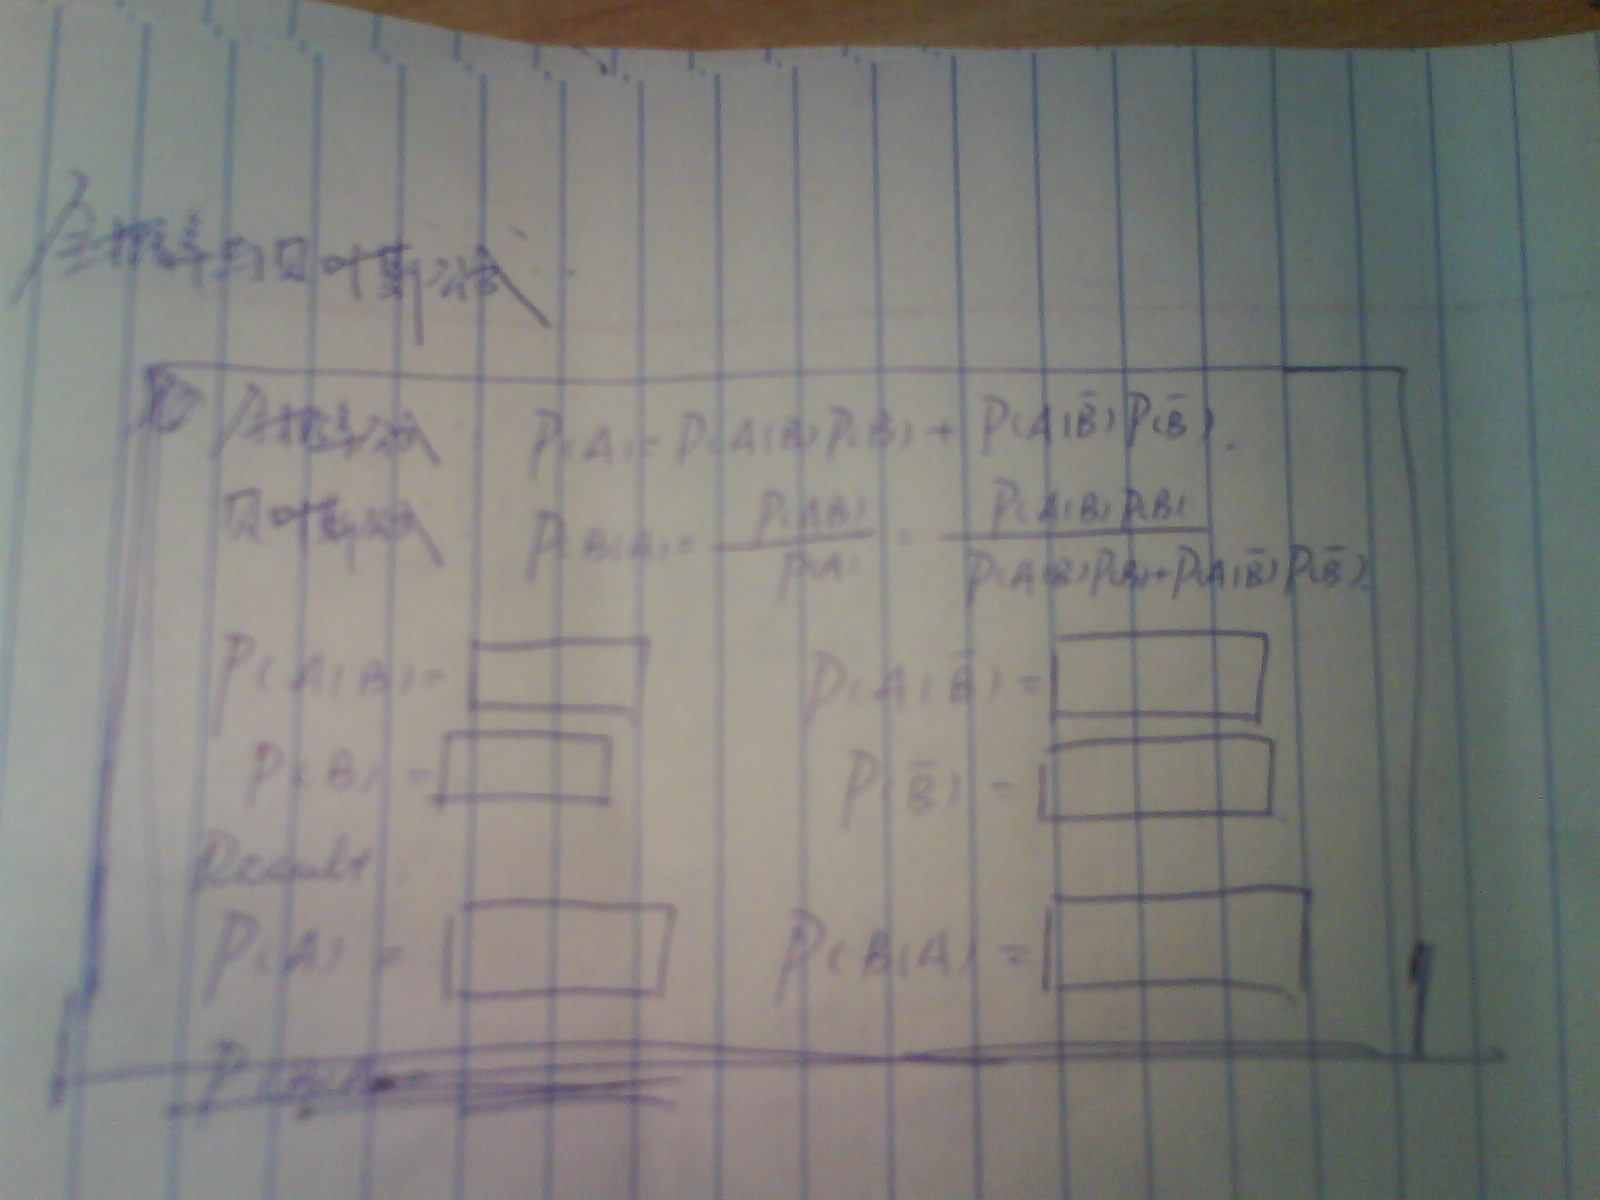
\includegraphics[width=\textwidth]{probability.ps}
\end{frame}

\begin{frame}
  \frametitle{正态分布\&图片工具}
  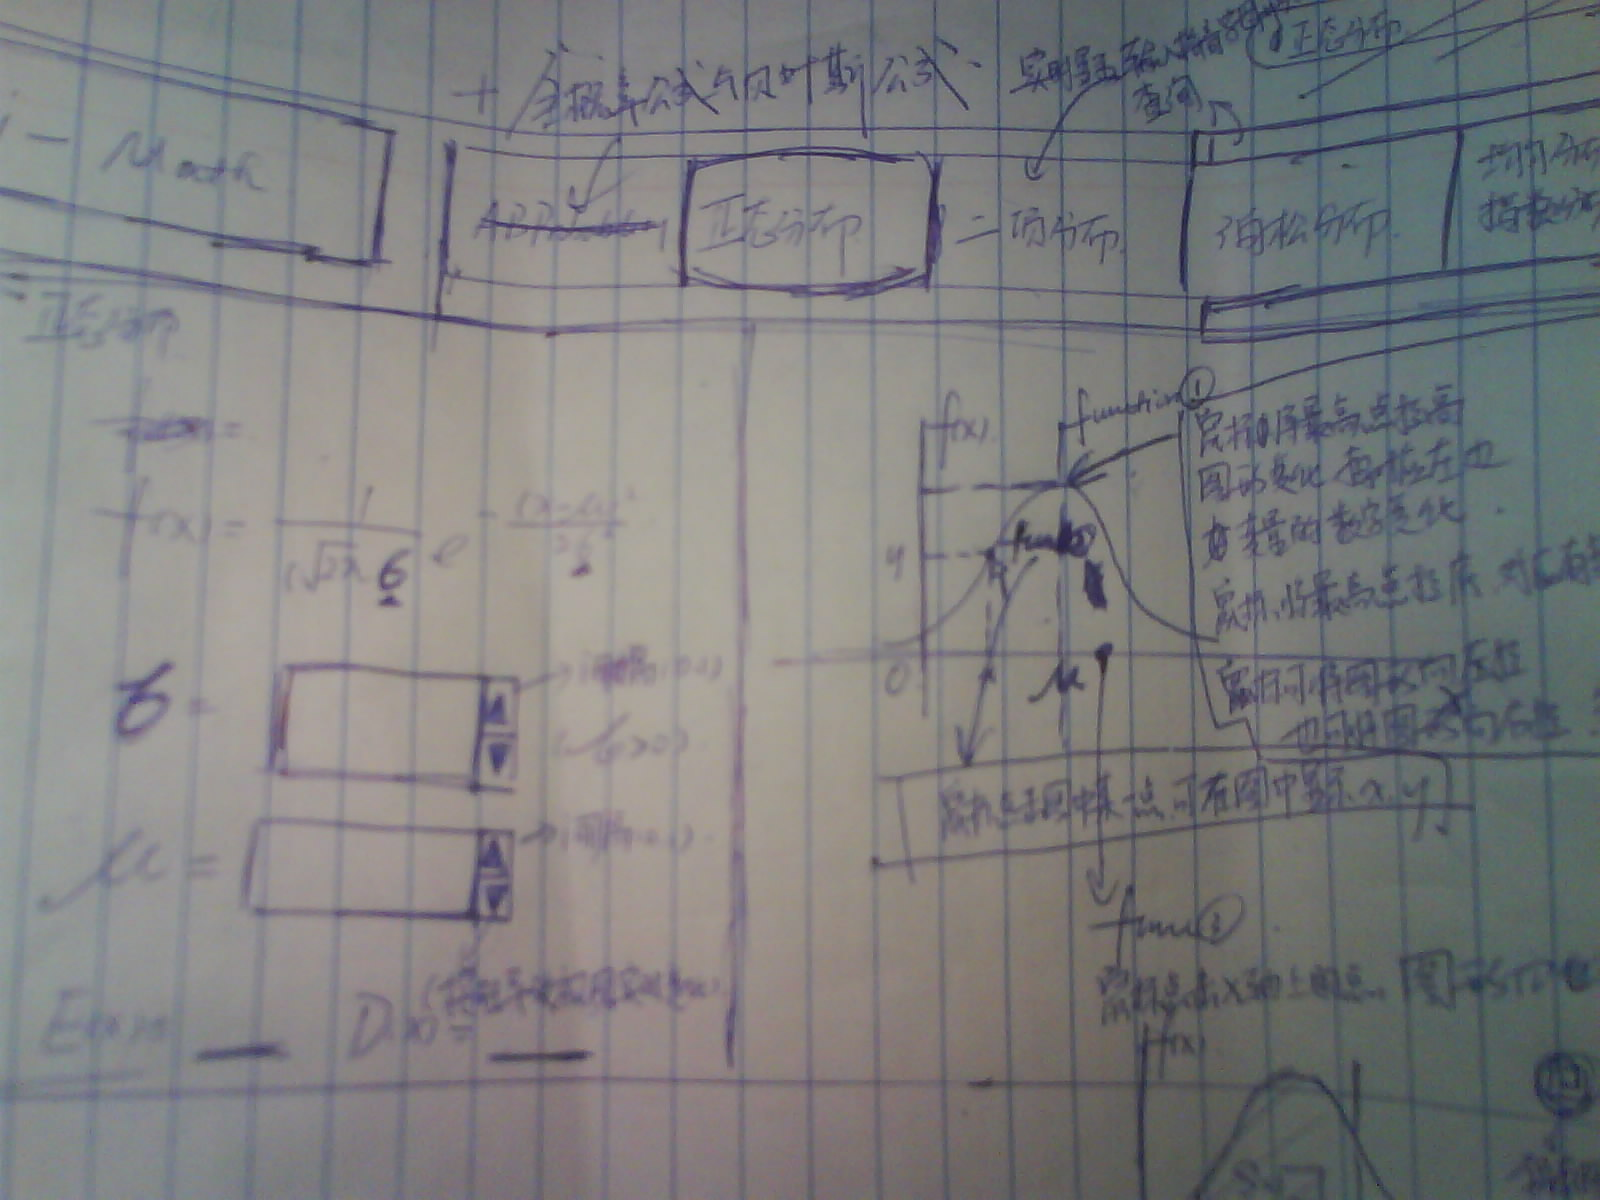
\includegraphics[width=\textwidth]{imageGadget.ps}
\end{frame}

\begin{frame}
  \frametitle{二项分布}
  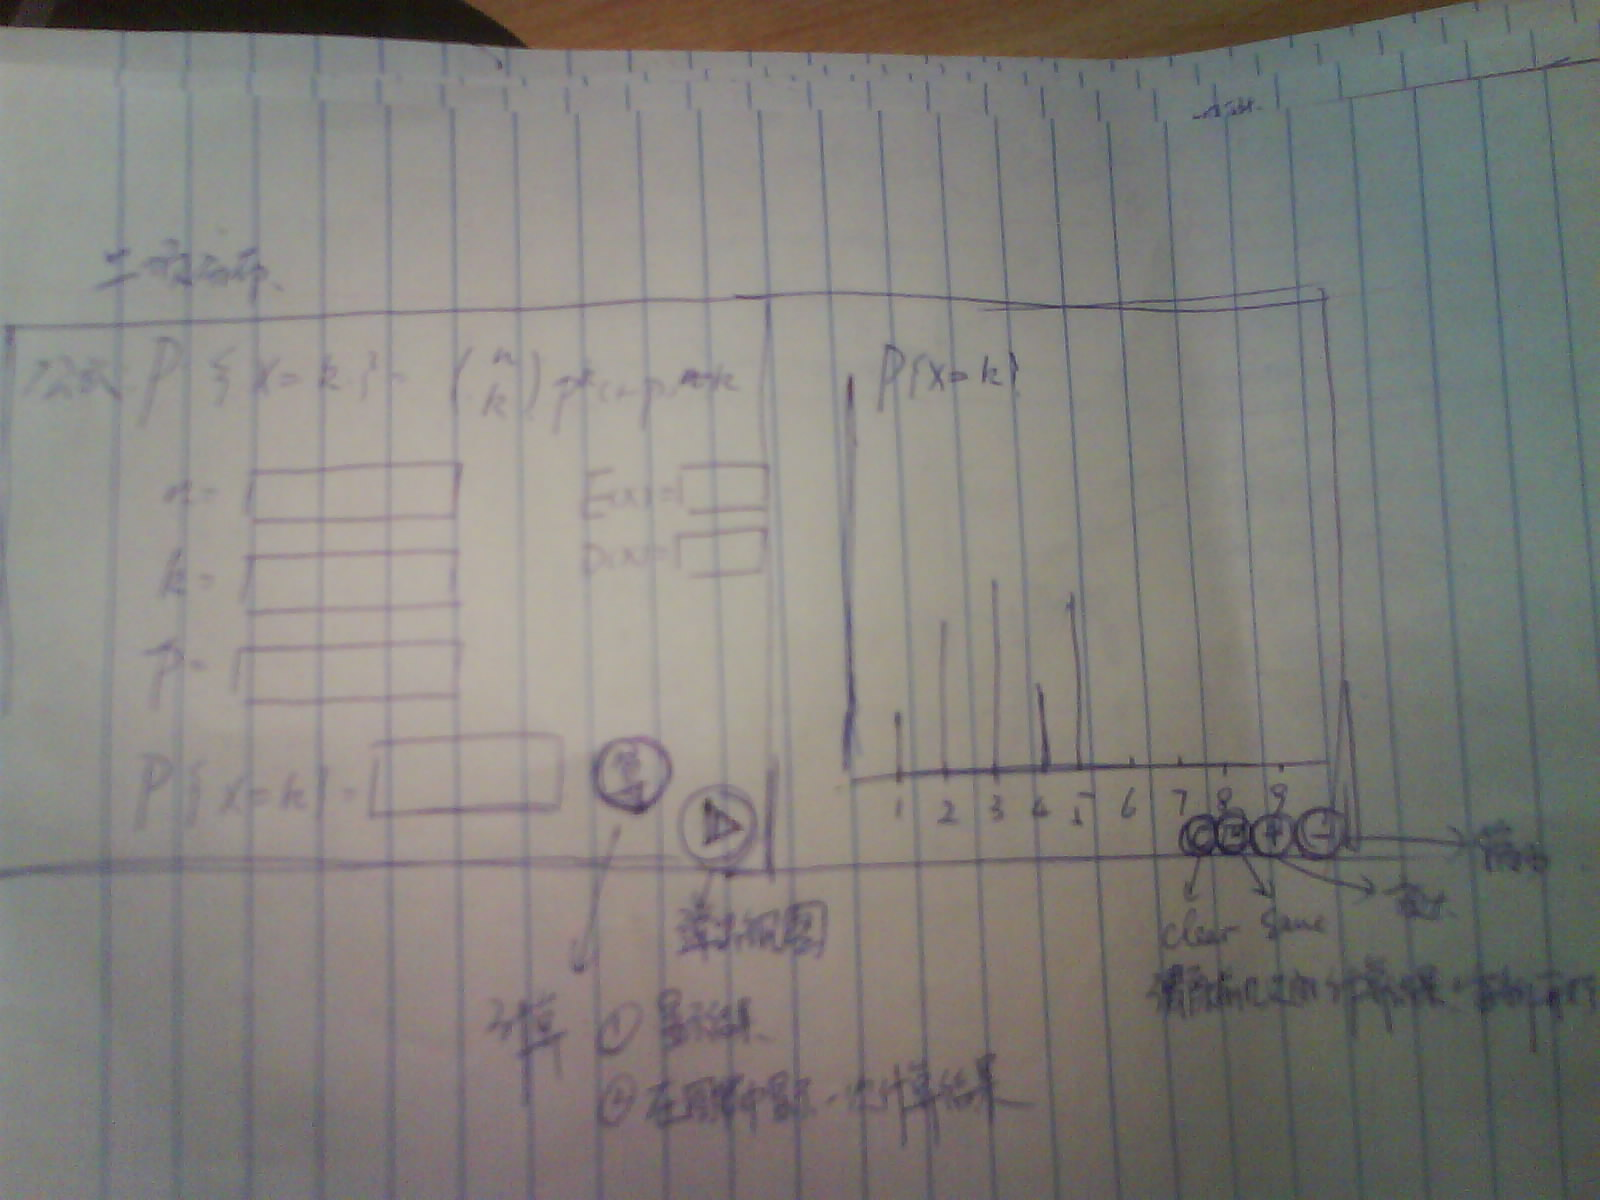
\includegraphics[width=\textwidth]{binomial-distribution.ps}
\end{frame}

\begin{frame}
  \frametitle{泊松分布}
  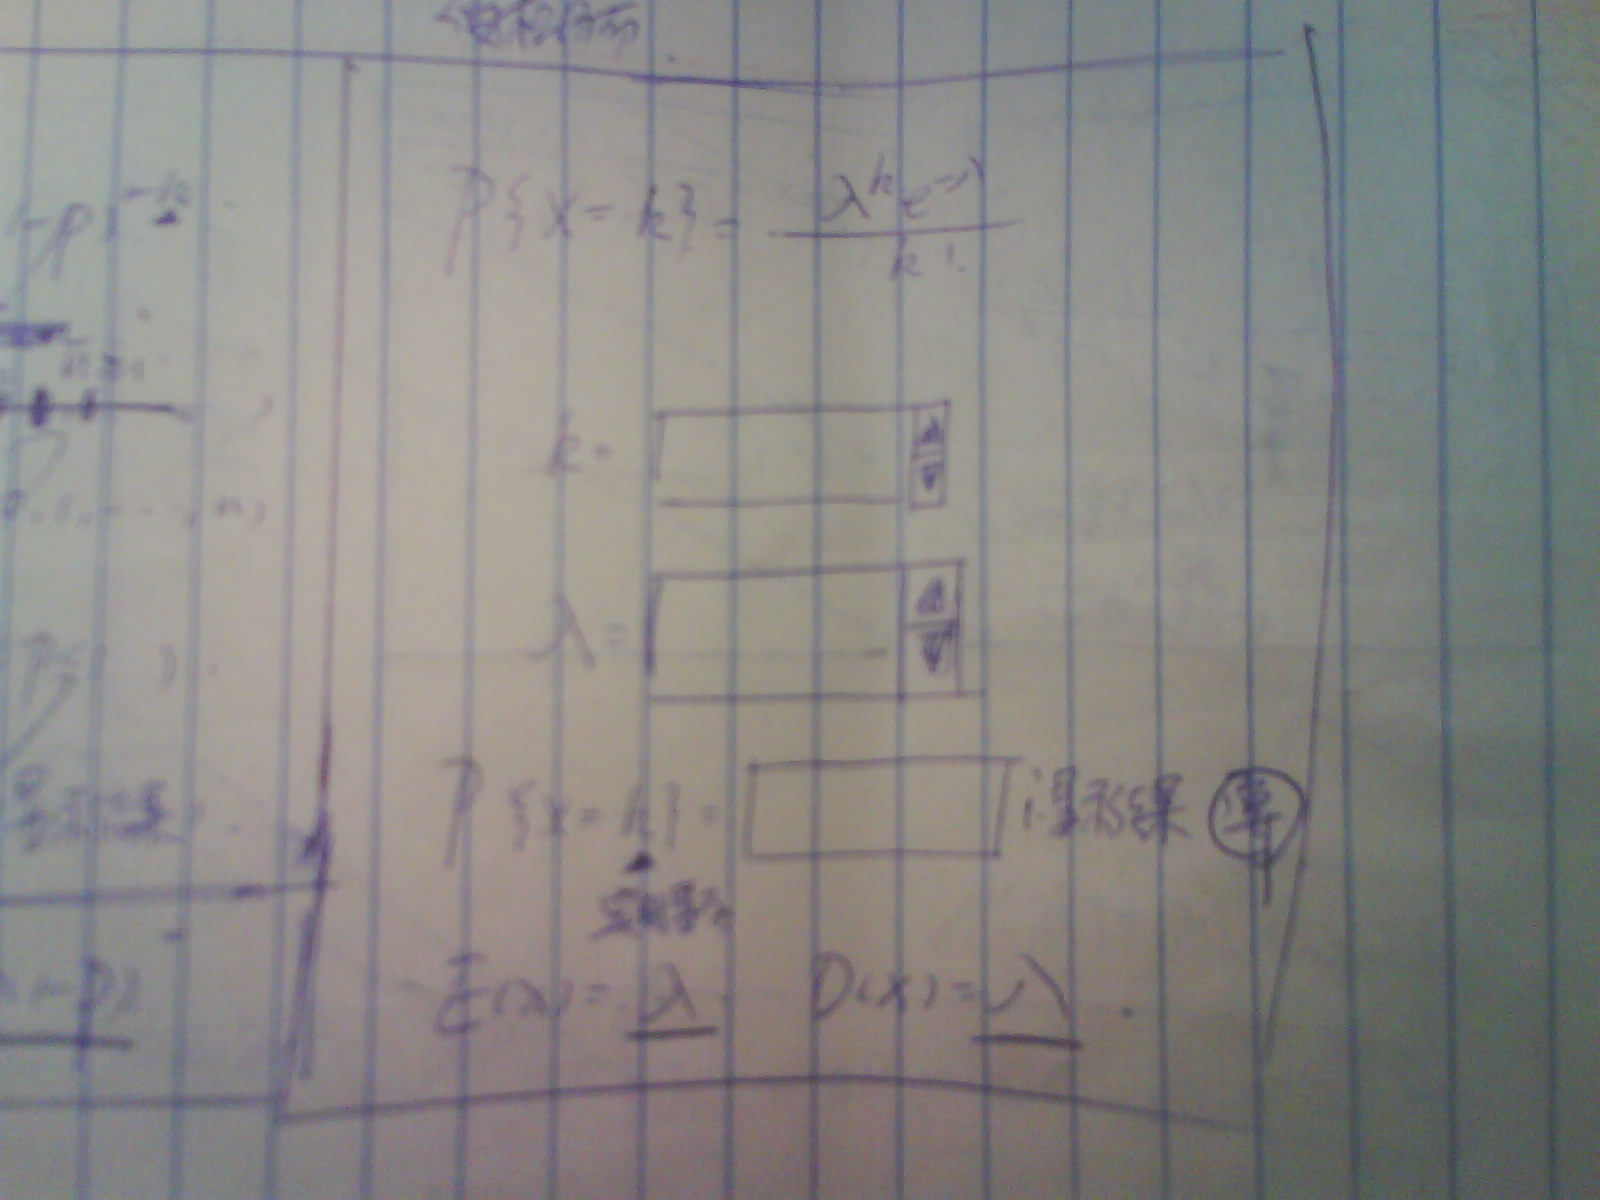
\includegraphics[width=\textwidth]{poisson-distribution.ps}
\end{frame}


\subsection{架构方面}

\begin{frame}
  \frametitle{Gadget引擎}
\begin{itemize}
 \item 测试方式:
\href{http://i-math.appspot.com/ifr.action?url=http://i-math.appspot.com/gadgets/add-gadget/add-gadget.xml}{http://i-math.appspot.com/ifr.action?url=http://i-math.appspot.com/gadgets/add-gadget/add-gadget.xml}
\item 引入Caja
  \end{itemize}
\end{frame}

\begin{frame}
  \frametitle{GadgetContainer核心}
\begin{itemize}
 \item 充分的缓存系统
\item Gadget互操作实现
\item 引入拖拽支持
\end{itemize}
\end{frame}

\begin{frame}
  \frametitle{核心}
\begin{itemize}
\item 基本架构搭建
\item 引入基于JPA+Datanucleus的数据库支持
\item 引入个性化支持
\item 引入结果缓存系统
\end{itemize}
\end{frame}

\section{结语}

\begin{frame}
%   \frametitle{谢谢}
\begin{center}
希望大家给予我们支持
\end{center}
\end{frame}

\end{document}
